
\section{Aufbau und Durchführung}
\label{sec:Durchführung}

\subsection{Aufbau}

Gearbeitet wird mit einer Grundplatte wie sie in Abbildung \ref{df:1} zu sehen ist.
\begin{figure}[H]
  \centering
  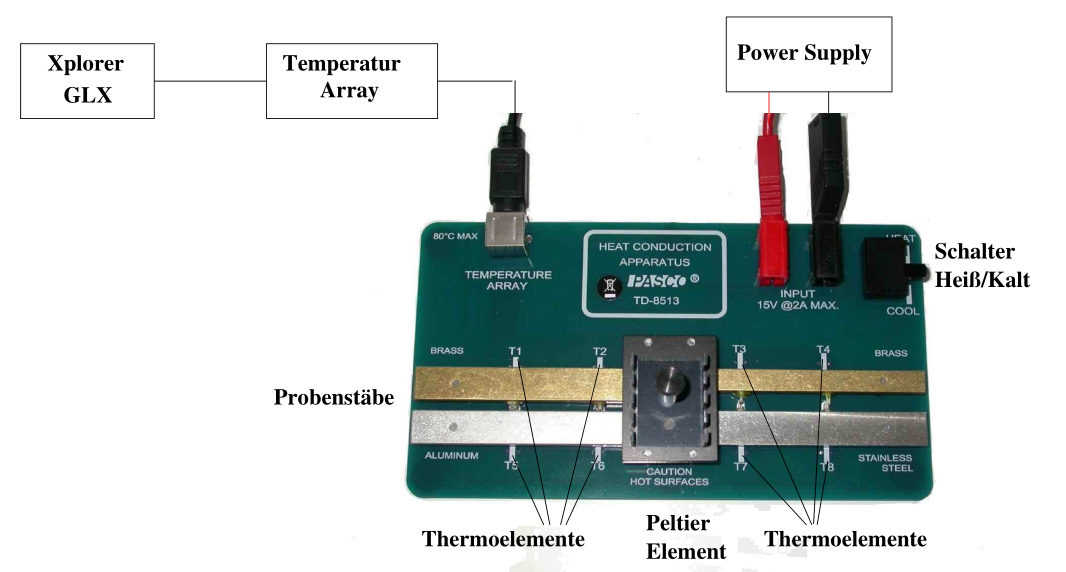
\includegraphics[height=6cm]{aufbau.png}
  \caption{Versuchsaufbau zur Untersuchung von Wärmeleitung. \cite{sample}}
  \label{df:1}
\end{figure}
Auf ihr befinden sich vier Probenstäbe, einer aus Aluminium, zwei aus Messing unterschiedlicher Ausdehnung und einer aus Edelstahl.
Um diese zu heizen, werden sie einseitig an ein Peltier-Element angeschlossen.
Dieses wird an eine Stromquelle angeschlossen.
Das Peltier-Element kann bei eingeschalteter Stromquelle je nach Stromrichtung basierend auf dem Peltier-Effekt als Wärmequelle dienen oder der Umgebung Wärme entziehen.
Mittels HEAT- und COOL-Kippschalter kann der gewünschte Effekt eingestellt werden.
Auf den Probenstäben sind jeweils zwei im Abstand $\increment x$ platzierte Thermoelemente, welche alle mit einem Temperaturarray verbunden sind.
Über den Xplorer GLX können die Temperaturdaten ausgelesen, geplottet und zum Drucken bereitgestellt werden.
Während des Versuchs werden die Probenstäbe über Abdeckkörper aus Schaumstoff hinreichend thermisch isoliert.

\subsection{Durchführung}

\subsubsection{Statische Methode}

Zunächst werden die abgedeckten Probenstäbe über das Peltier-Element aufgeheizt, bis das Thermoelement T7 eine Temperatur von etwa $T_7 \approx \SI{45}{\celsius}$ erreicht.
Während dieses Aufheizvorgangs werden alle Temperaturen vom Xplorer GLX aufgenommen.
Über ihn werden die Temperaturen $T_1$ und $T_4$, und $T_5$ und $T_8$ jeweils gegen die Zeit graphisch dargestellt.
Ebenfalls werden die Temperaturdifferenzen $T_7-T_8$ und $T_2-T_1$ gegen die Zeit abgetragen.
Diese Messreihe dient jedoch nur, um qualitative Aussagen über die Wärmeleitfähigkeit der Proben zu gewinnen.
Für quantitative Ergebnisse wird das Angström-Verfahren verwendet.

\subsubsection{Dynamische Methode: Das Angström-Verfahren}

Hierzu werden die Probenstäbe, nachdem sie runtergekühlt worden sind, in einer Periode von $T'=\SI{80}{\second}$ aufgeheizt und abgekühlt.
Dies geschieht über mindestens zehn Perioden.
Die Temperaturverläufe des breiten Messingstabes $(T_1,T_2)$ und des Aluminiumstabes $(T_5,T_6)$ werden nun gegen die Zeit aufgetragen und ausgedruckt.
Nach erneutem Kühlen der Proben wird dieses Verfahren mit einer Periode von $T' = \SI{200}{\second}$ wiederholt.
Diesmal wird der Temperaturverlauf des Edelstahlstabes $(T_7,T_8)$ geplottet.
Aus diesen Daten kann auf die Ausbreitungsgeschwindigkeit und somit auf die Wärmeleitfähigkeit der Proben geschlossen werden.
